\documentclass[tikz,border=10pt]{standalone}
\usepackage{amsmath,amssymb}
\usepackage{tikz}
\usepackage{pgfplots}
\pgfplotsset{compat=1.18}
\usetikzlibrary{arrows.meta,calc,patterns,positioning,shapes,decorations.markings,backgrounds,fit,intersections}

% Atlas colors
\definecolor{AtlasTeal}{HTML}{5BA4A4}
\definecolor{AtlasTealDark}{HTML}{4A8F8F}
\definecolor{AtlasTealLight}{HTML}{E8F4F4}
\definecolor{AtlasDeep}{HTML}{2C5F5F}
\definecolor{AtlasSage}{HTML}{7BAE7F}
\definecolor{AtlasSageLight}{HTML}{EDF5EE}
\definecolor{AtlasWarm}{HTML}{D4A853}
\definecolor{AtlasWarmLight}{HTML}{FDF6E8}
\definecolor{AtlasBorder}{HTML}{E8E5E1}

\begin{document}
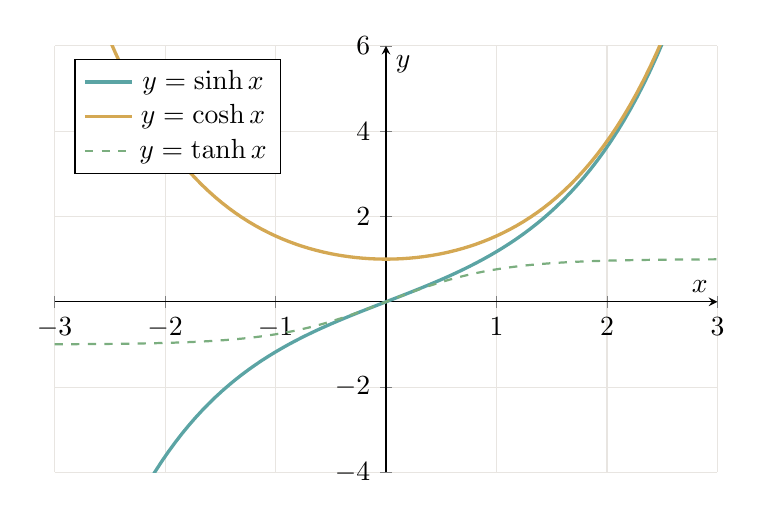
\begin{tikzpicture}
  \begin{axis}[
    width=10cm, height=7cm,
    axis lines=middle,
    xlabel={$x$}, ylabel={$y$},
    xmin=-3, xmax=3, ymin=-4, ymax=6,
    samples=100,
    legend pos=north west,
    grid=major,
    grid style={AtlasBorder, thin},
  ]
    \addplot[AtlasTeal, very thick, domain=-3:3] {(exp(x)-exp(-x))/2};
    \addlegendentry{$y = \sinh x$}
    \addplot[AtlasWarm, very thick, domain=-3:3] {(exp(x)+exp(-x))/2};
    \addlegendentry{$y = \cosh x$}
    \addplot[AtlasSage, thick, dashed, domain=-3:3] {(exp(x)-exp(-x))/(exp(x)+exp(-x))};
    \addlegendentry{$y = \tanh x$}
  \end{axis}
\end{tikzpicture}
\end{document}
